\chapter{Bilan}

\section{Bilan du travail r\'ealis\'e}

\subsection{R\'ecapitulatif du projet}

La figure~\ref{figure:yuukouEtYuukouII} permet de donner une vue d'ensemble sur les principales fonctionnalit\'es dont le projet dispose.
Les cadres pleins repr\'esentent des fonctionnalit\'es dont le principe a \'et\'e repris de {\Yuukou}, les cadres en pointill\'es quant \`a eux, repr\'esentent les nouvelles fonctionnalit\'es qu'apporte \YuukouII.

\begin{figure}[!ht]
	\centering
	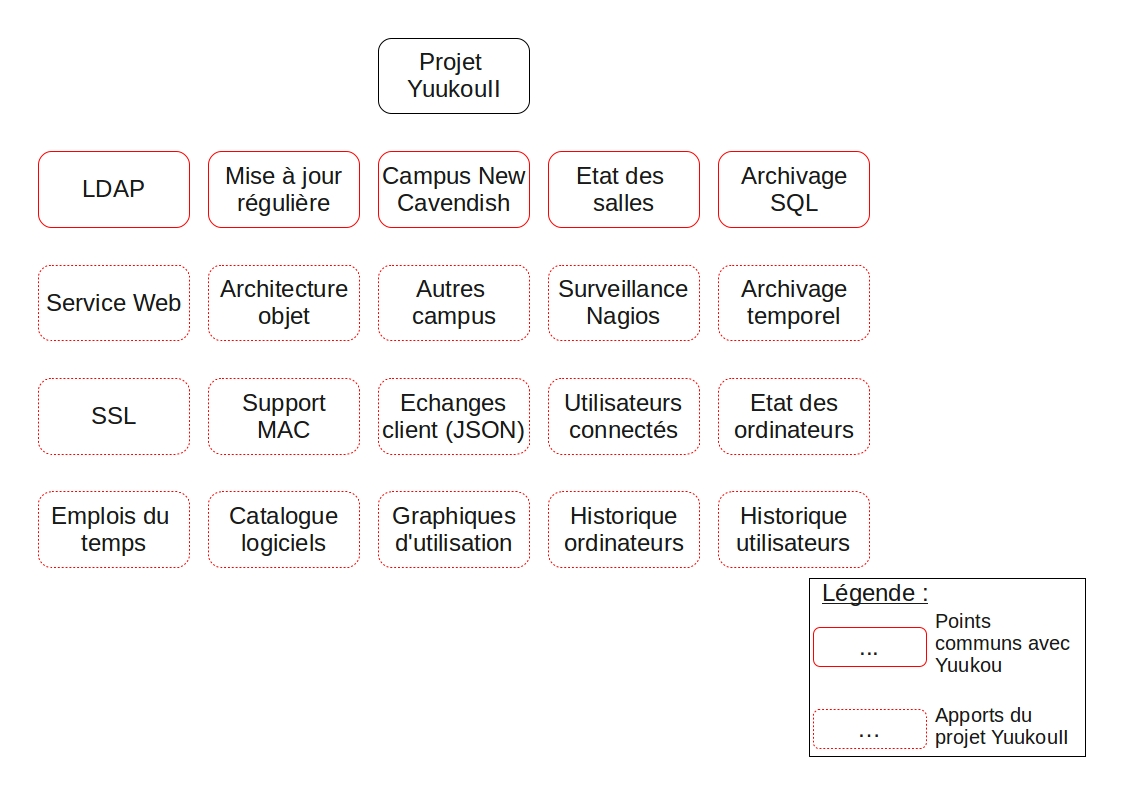
\includegraphics[scale=0.375]{yuukouEtYuukouII.jpg}
	\caption{R\'ecapitulatif des fonctionnalit\'es reprises de {\Yuukou} et les nouvelles de \YuukouII}
	\label{figure:yuukouEtYuukouII}

\end{figure}

\subsection{Calendrier du stage}
Arriv\'ee : Lundi 13 F\'evrier
D\'epart : Lundi 4 Juin

semaine 1 : Arriv\'ee et d\'ecouverte du projet, premier entretien avec l'\'equipe technique et leurs attentes
semaine 2 : D\'ecouverte des services Web et choix des outils utilis\'es
semaine 3 : Conception de la base de donn\'ees et d\'ebut d'impl\'ementation du cycle principal de l'application
semaine 4 : fin d'impl\'ementation du cycle principal
semaine 5 : Mise en place de l'emploi du temps + mise en place de SSL
semaine 6 : D\'eveloppement des premi\`eres m\'ethodes Web + fin de mise en place de SSL
semaine 7 : Mise en place du syst\`eme JSON
semaine 8 : 
semaine 9 : 
semaine 10 : D\'ebut de r\'edaction du rapport
semaine 11 : 
semaine 12 : 
semaine 13 : R\'ecup\'eration du catalogue de logiciels de M\'ediaWiki
semaine 14 : Ajout de m\'ethodes Web et am\'elioration du chargement de la base de donn\'ees
semaine 15 : r\'edaction du rapport de stage et maintenance des fonctionnalit\'es du service Web
semaine 16 : fin d'\'ecriture du rapport de stage

\subsection{R\'esultat pour l'Universit\'e}

\subsection{Am\'eliorations possibles}

Le projet {\YuukouII} est loin d'\^etre fini m\^eme si fonctionnel \`a l'heure actuelle.
Il reste diverses fonctionnalit\'es \`a d\'evelopper.
Une de ces fonctionnalit\'es serait de rajouter une s\'ecurit\'e lors de l'acc\`es aux m\'ethodes du service Web par le client.
En effet, il serait int\'eressant que le client s'authentifie.
De ce fait, deux r\^oles pourraient \^etre d\'efinis : administrateur et utilisateur.
Avec cette m\'ethode, un utilisateur ne pourrait jamais se servir d'une m\'ethode dite priv\'ee car actuellement, si un client d\'eveloppe son propre programme pour acc\'eder au service Web {\YuukouII}, une fois le protocole SSL\protect\footnote{\textit{Secure Sockets Layer}} en place, rien ne l'emp\^eche d'utiliser les fonctions qu'il veut.

Des am\'eliorations peuvent aussi \^etre port\'ees sur la fa\c{c}on dont RRDtool a \'et\'e mis en place.
Il ne s'agit que d'un essai pour tester les possibilit\'es, mais il serait int\'eressant de l'int\'egrer pleinement au service Web et surtout au cycle principal d'ex\'ecution.


\section{Bilan humain}

\section{Bilan p\'edagogique}

\clearpage
